\section{Memória}

No contexto de FSMs, a memória é um elemento fundamental para o armazenamento de informações e estados. Existem diversos tipos de elementos de memória, construidos de forma hierárquica em complexidade, cada um com suas características e aplicações específicas. 

Nesta seção, serão abordados os principais tipos de elementos de memória utilizados em FSMs, incluindo flip flops do tipo SR, JK, D e T, além de registradores.

\subsection{Latch SR}

O latch SR (Set-Reset) é o elemento de memória mais simples, composto por duas portas lógicas interligadas por realimentação.

Ele possui duas entradas principais:
\begin{itemize}
    \item $S$ (Set): força a saída para 1
    \item $R$ (Reset): força a saída para 0
\end{itemize}

Seu comportamento pode ser descrito pela seguinte tabela de transição de estados:

\begin{center}
\begin{tabular}{c c | c}
S & R & $Q_{t+1}$ \\
\hline
0 & 0 & $Q_t$ \\
0 & 1 & 0 \\
1 & 0 & 1 \\
1 & 1 & indefinido
\end{tabular}
\end{center}

onde $Q_t$ representa o estado atual e $Q_{t+1}$ o próximo estado do sistema.

Observa-se que, na ausência de estímulos ($S = R = 0$), o circuito preserva seu estado anterior. Essa propriedade de retenção de informação caracteriza um elemento de memória.

Existem duas implementações clássicas do latch SR, baseadas em portas NOR e NAND:

\begin{figure}[H]
    \centering
    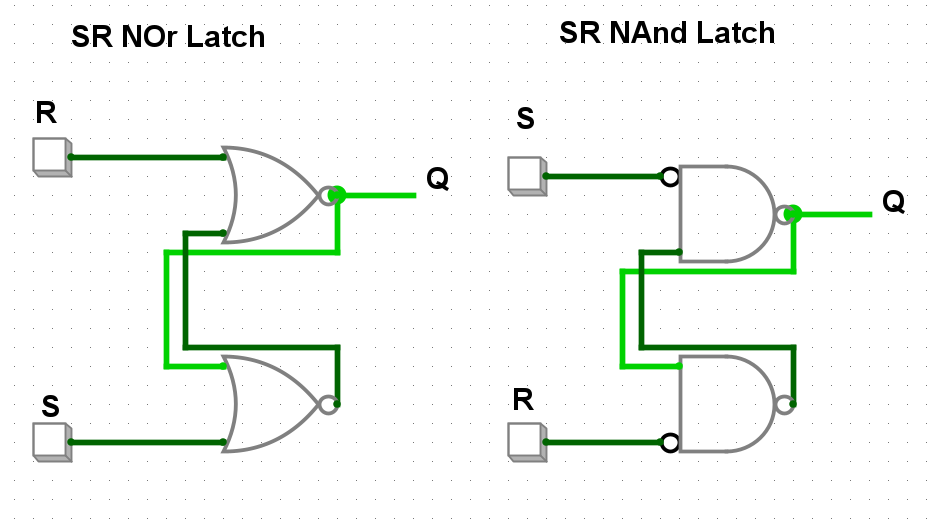
\includegraphics[width=0.6\linewidth]{images/sr-latch-circuit.png}
    \caption{Implementações do latch SR com portas NOR e NAND}
    \label{fig:sr-latch-circuit}
\end{figure}

Neste trabalho, será utilizada a implementação com portas NOR.

Utilizando redstone, é possível construir um latch SR equivalente:

\begin{figure}[H]
    \centering
    \includegraphics[width=0.8\linewidth]{images/sr-nor-latch-redstone.png}
    \caption{Latch SR implementado no Minecraft}
    \label{fig:sr-nor-latch-redstone}
\end{figure}

A condição $S = R = 1$ é considerada inválida pois força simultaneamente as duas saídas do circuito, violando a relação complementar entre $Q$ e $\lnot Q$. Em circuitos reais, isso pode levar a um estado indeterminado ou metaestável, no qual o valor final não é previsível.

Pode-se adicionar um controle de clock a partir de duas portas AND, recebendo as entradas $S$ e $R$ e o pulso de clock.

\begin{figure}[H]
    \centering
    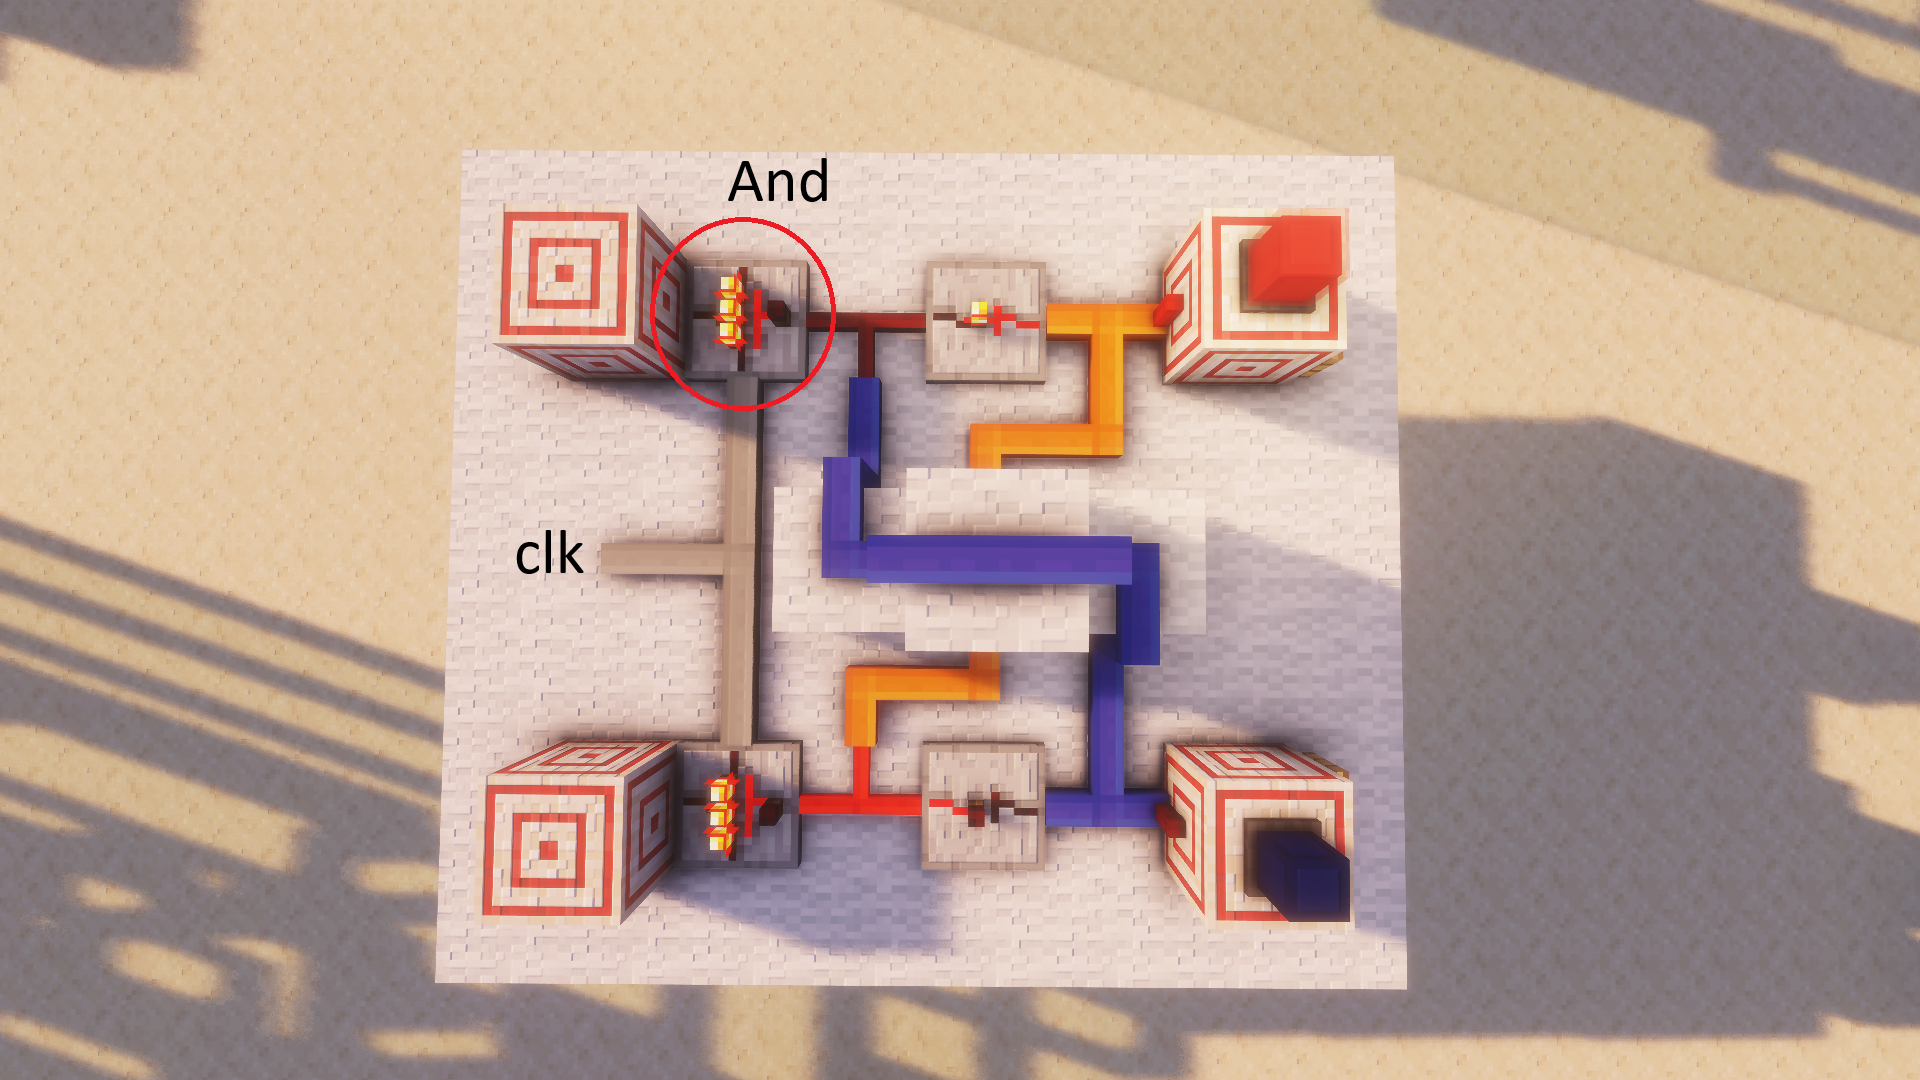
\includegraphics[width=0.8\linewidth]{images/sr-nor-latch-redstone-clock.png}
    \caption{Latch SR implementado no Minecraft com controle de clock}
    \label{fig:sr-nor-latch-redstone-clock}
\end{figure}
\subsection{Flip-Flop JK}

O flip-flop JK é uma evolução do latch SR que resolve o estado inválido.

Entradas:
\begin{itemize}
    \item $J$ (Set)
    \item $K$ (Reset)
\end{itemize}

Tabela de transição:

\begin{center}
\begin{tabular}{c c | c}
J & K & $Q_{t+1}$ \\
\hline
0 & 0 & $Q_t$ \\
0 & 1 & 0 \\
1 & 0 & 1 \\
1 & 1 & $\overline{Q_t}$
\end{tabular}
\end{center}

A pode ser feita da seguite forma: 

\begin{figure}[H]
    \centering
    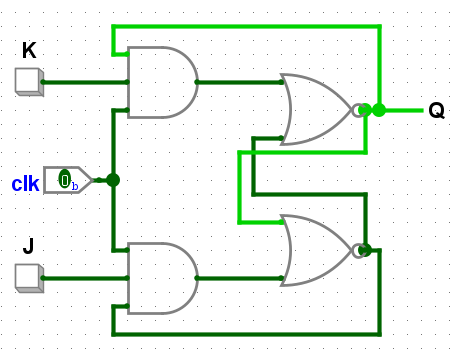
\includegraphics[width=0.6\linewidth]{images/JK-FF-circuit.png}
    \caption{Implementação do Flip Flop JK a partir do SR Nor Latch no Logisim Evolution}
    \label{fig:JK-FF-circuit}
\end{figure}

\begin{figure}[H]
    \centering
    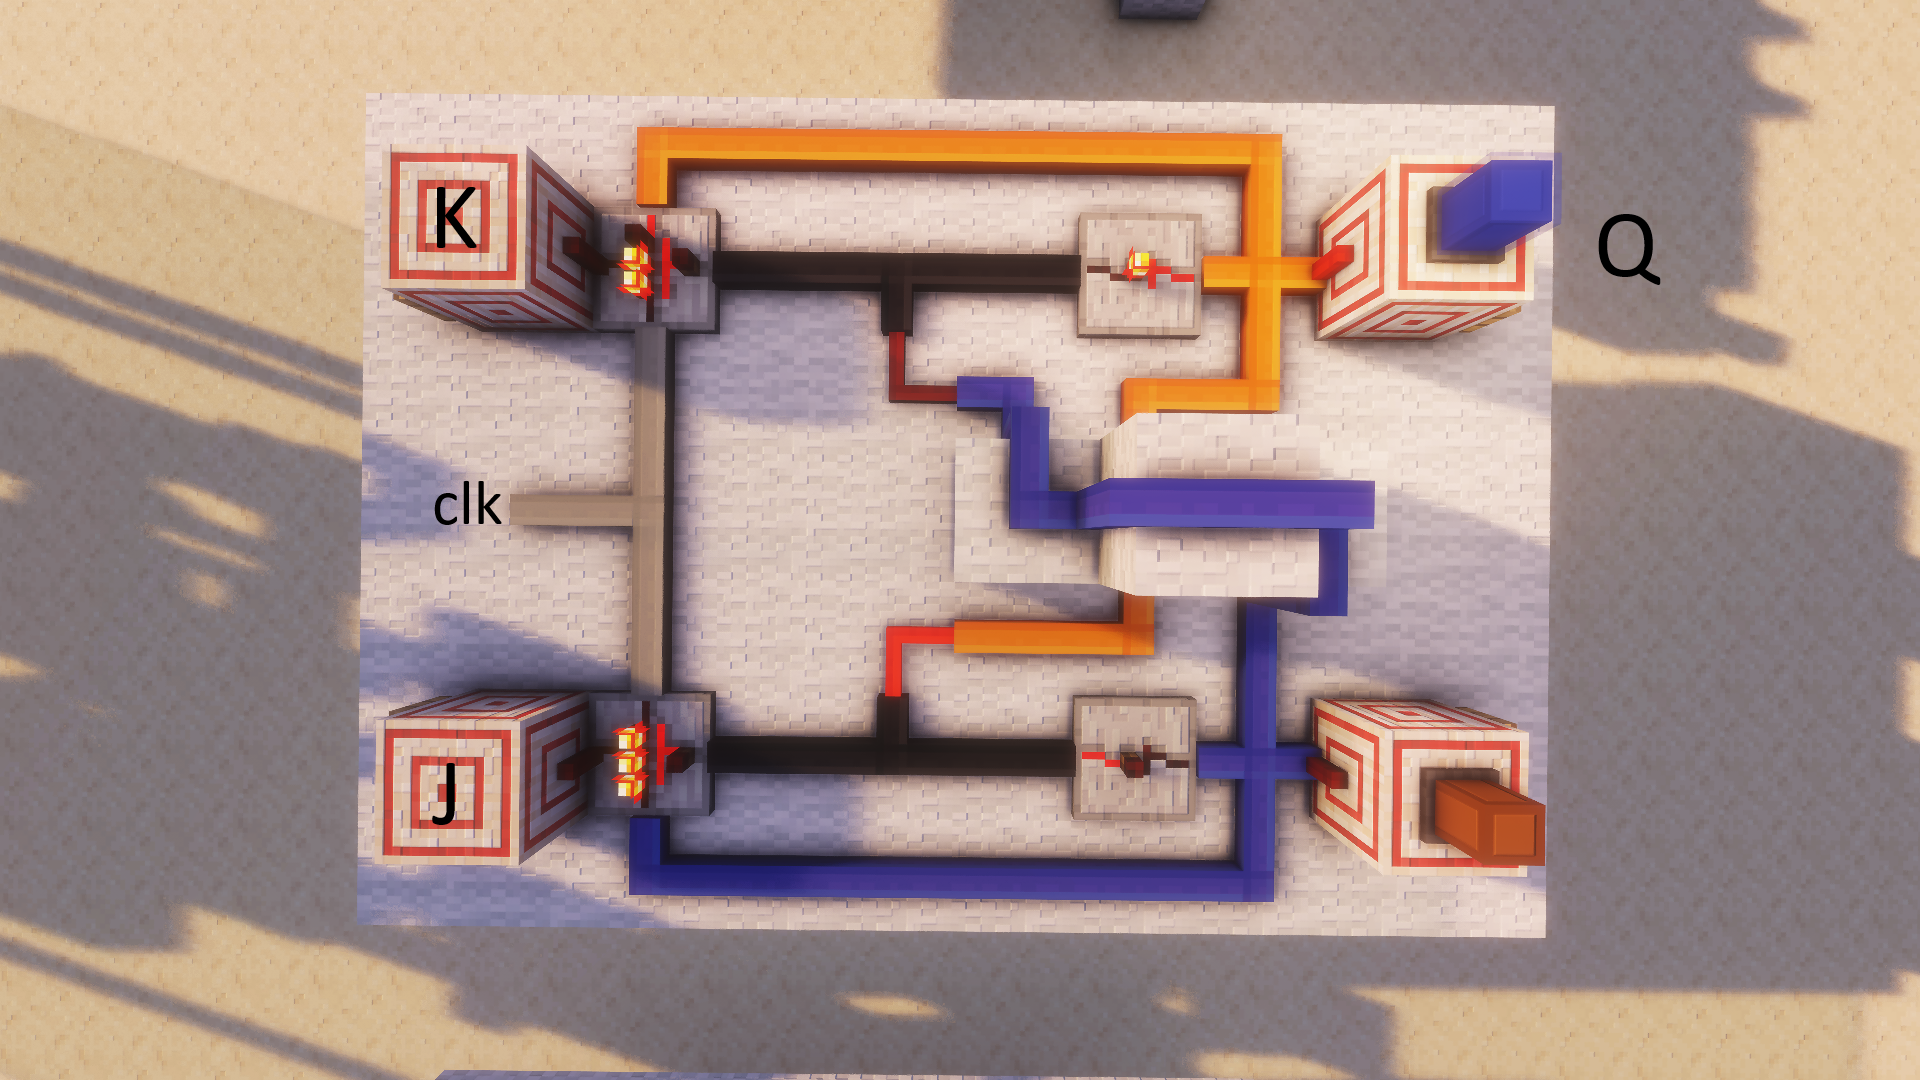
\includegraphics[width=0.8\linewidth]{images/JK-FF-redstone.png}
    \caption{Implementação do Flip Flop JK a partir do SR Nor Latch no Minecraft}
    \label{fig:JK-FF-redstone}
\end{figure}

O estado $Q$ é atualizado apenas durante o nível ativo do sinal de clock. No entanto, quando $J = K = 1$, o circuito tende a alternar continuamente entre $Q$ e $\lnot Q$ devido à realimentação interna.

Para evitar esse comportamento, é necessário que a duração do pulso de clock ($t_{high}$) seja menor que o tempo total de propagação do circuito ($t_{loop}$):

\[
t_{high} < t_{loop}
\]

Nesse contexto, detectores de borda podem ser utilizados para transformar o sinal de clock em pulsos extremamente curtos, associados apenas às transições do sinal.

Dessa forma, garante-se que apenas uma transição de estado ocorra por pulso de clock, evitando múltiplas comutações indesejadas.

Esse problema é conhecido como \textit{race-around condition} e ocorre em implementações sensíveis ao nível do clock.
\subsection{Flip-Flop D}

O flip-flop D (Data) é o mais utilizado em sistemas digitais reais devido à sua simplicidade. Ele possui apenas uma entrada:

\begin{itemize}
    \item $D$: Data
\end{itemize}

\begin{center}
\begin{tabular}{c | c}
D & $Q_{t+1}$ \\
\hline
 0 & 0 \\
 1 & 1 \\
\end{tabular}
\end{center}

Ou seja, em $t+1$ o circúito assume o estado D.

\begin{figure}[H]
    \centering
    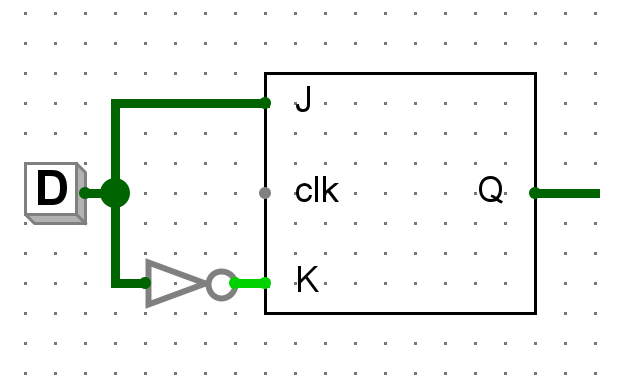
\includegraphics[width=0.5\linewidth]{images/D-FF.png}
    \caption{Implementação do Flip Flop tipo D a partir do Flip Flop JK}
    \label{fig:D-FF}
\end{figure}

Apesar de ser possível fazer esta implementação no Minecraft,

\begin{figure}[H]
    \centering
    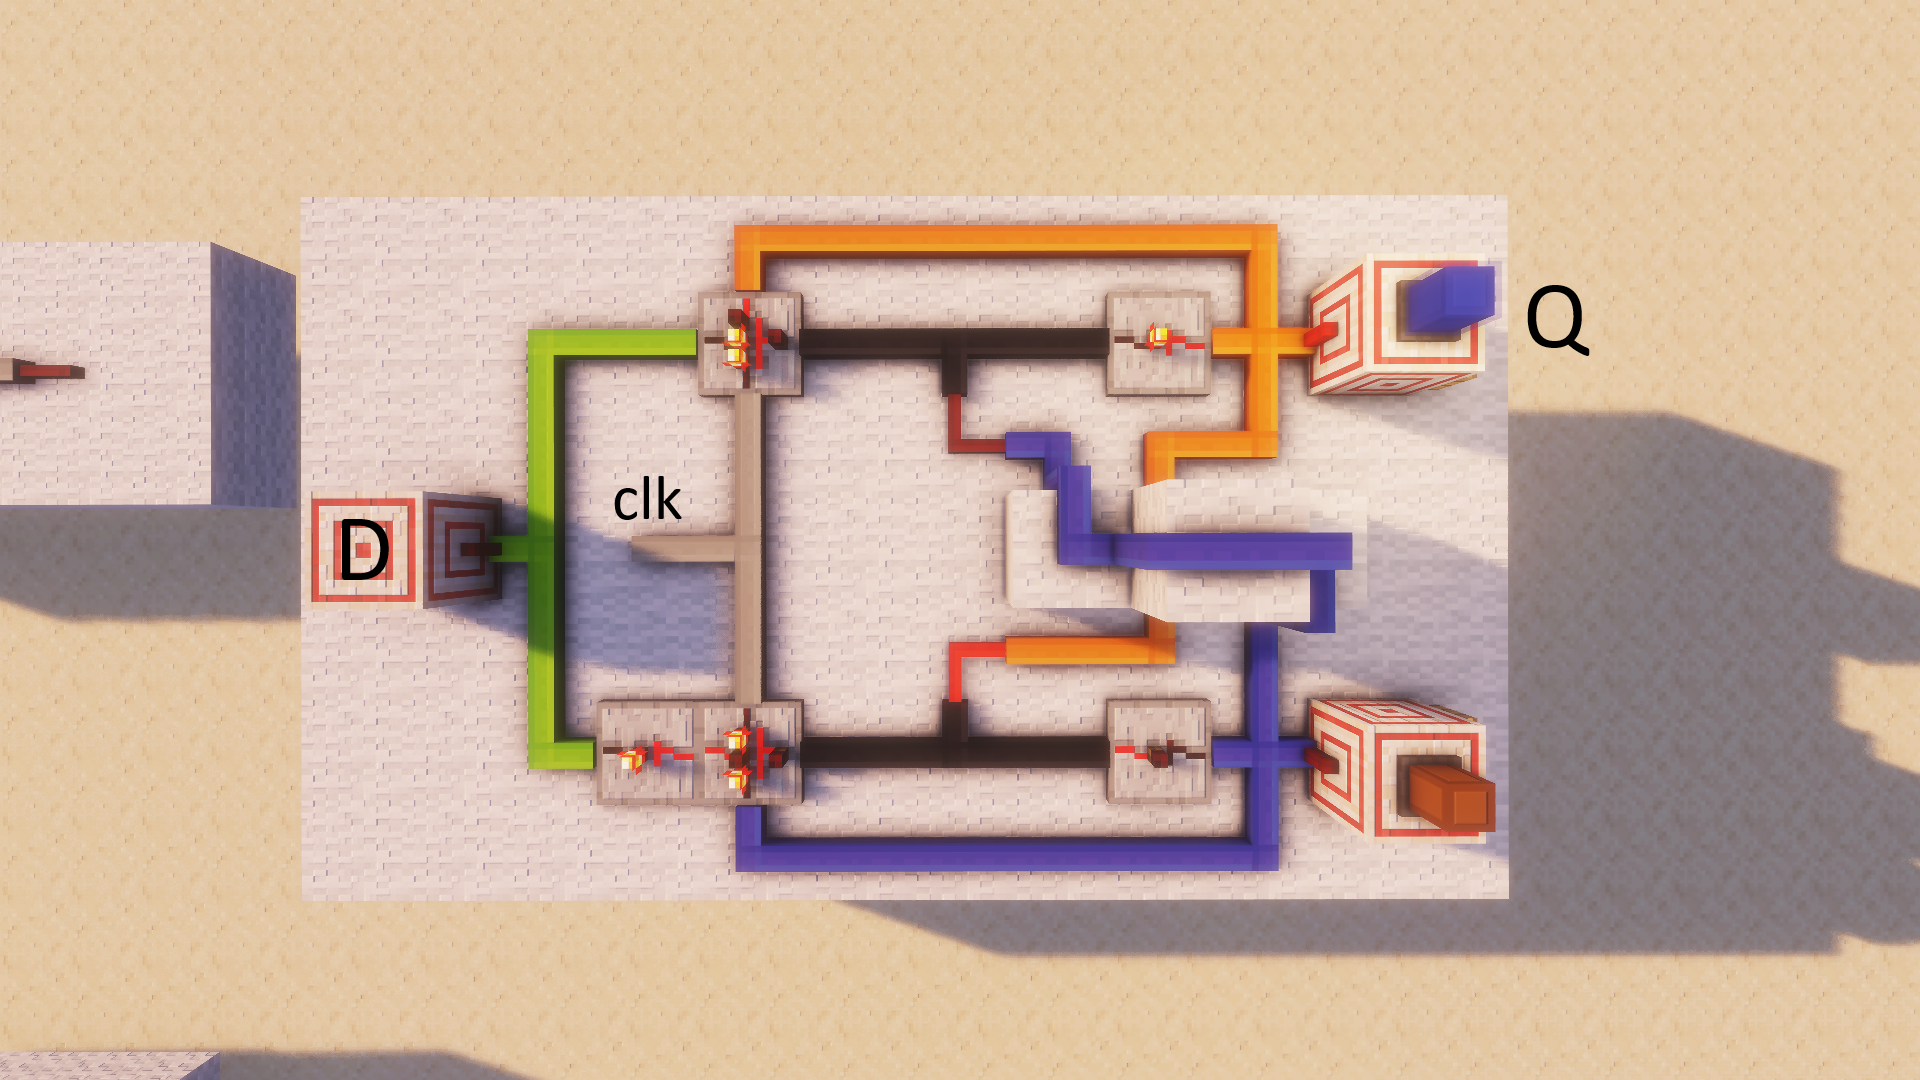
\includegraphics[width=0.8\linewidth]{images/D-FF-redstone-expanded.png}
    \caption{Implementação do Flip Flop tipo D a partir do Flip Flop JK em redstone}
    \label{fig:D-FF-redstone-expanded}
\end{figure}

tipicamente, aproveita-se da propiedade de trava dos repetidores de redstone para implementar o Flip Flop tipo D, na seguinte disposição:

\begin{figure}[H]
    \centering
    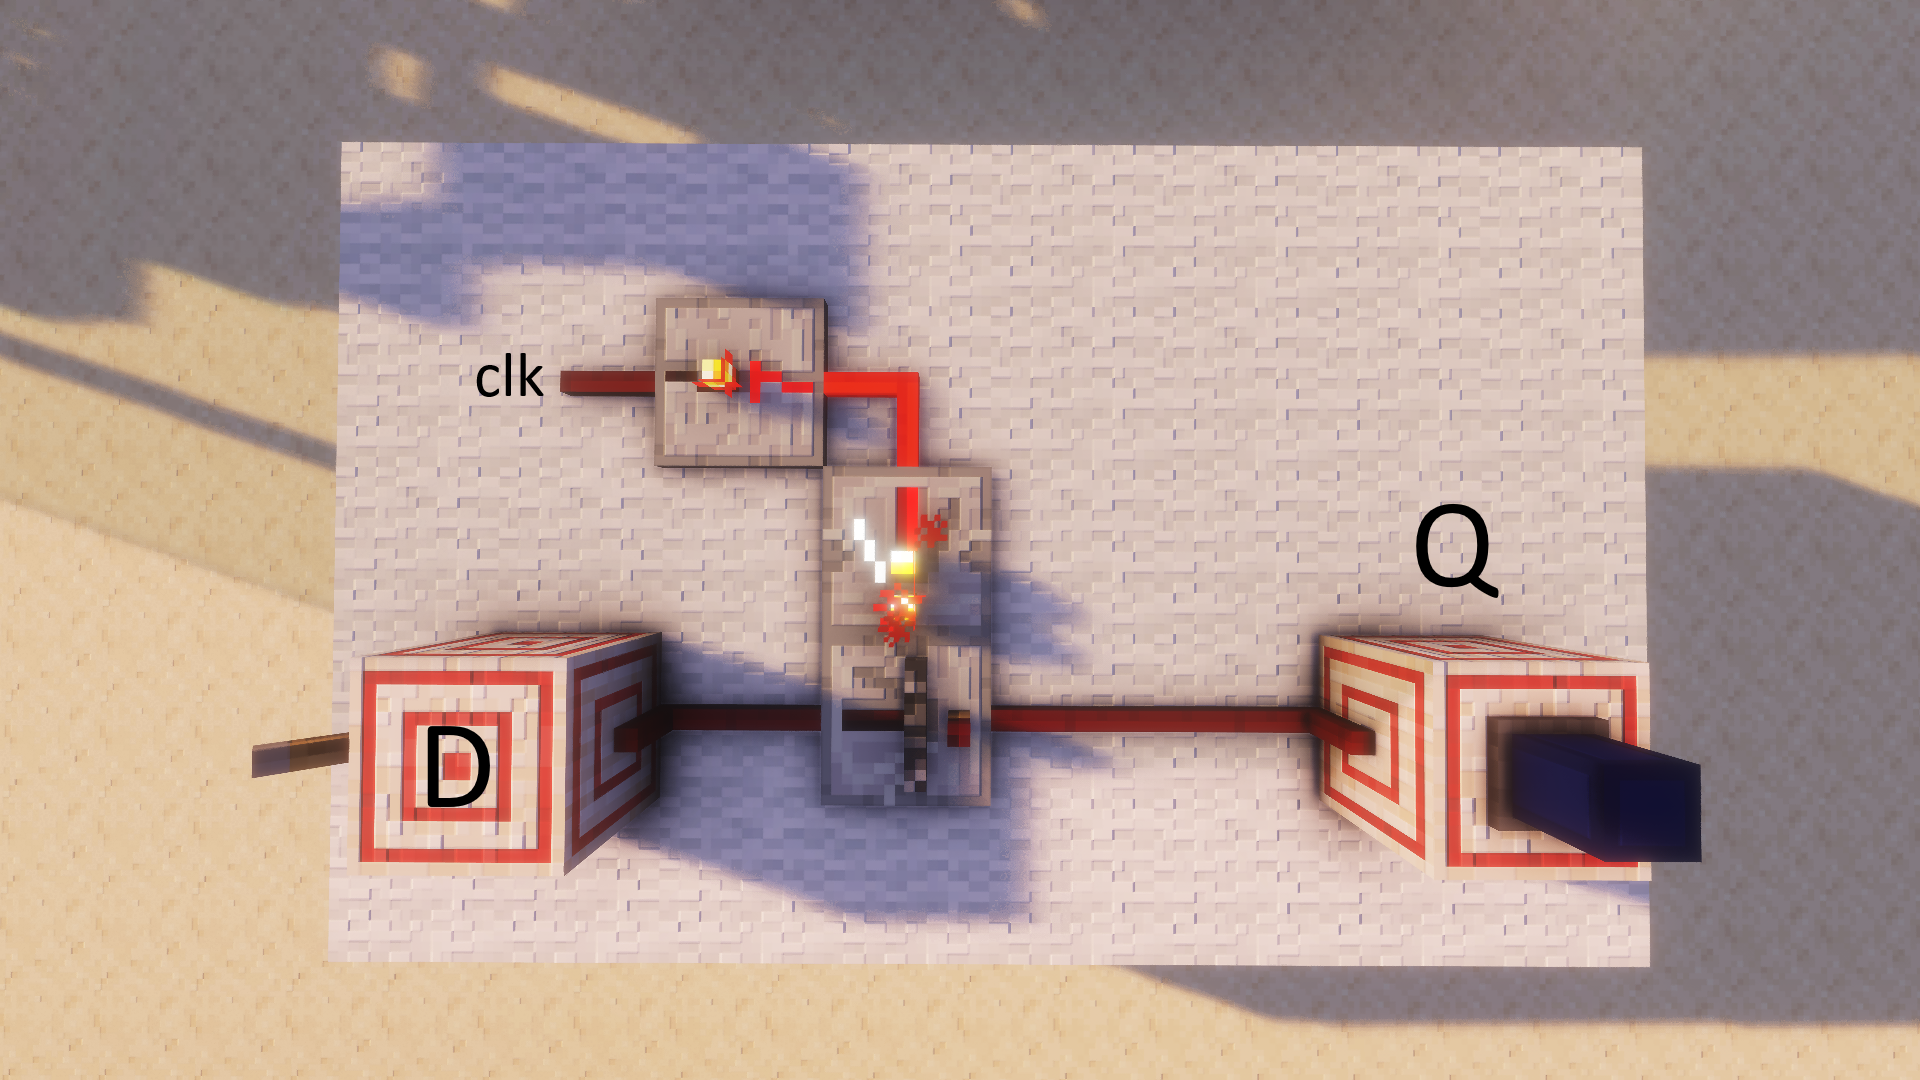
\includegraphics[width=0.8\linewidth]{images/D-FF-redstone.png}
    \caption{Implementação do Flip Flop tipo D a partir de repetidores de redstone}
    \label{fig:D-FF-redstone}
\end{figure}

De forma simplificada, enquanto $clk=0$ o repetidor trava no estado $Q$, quando o sinal de clock sobe, o repetidor é destravado e o estado de D é liberado para passar por ele. Assim, quando o clock desce, o repetidor trava no estado de $D$.

Entretanto, existe um atraso entre o clock e o lock efetivo do sistema. Observe o diagrama temporal desse sistema. No exemplo considerado, o clock possui período de $10$ Game Ticks e duty cycle de $50\%$. O repetidor está configurado para $1$ RT, e o portão NOT introduz um atraso de $1$ GT.

\begin{figure}[H]
    \centering
    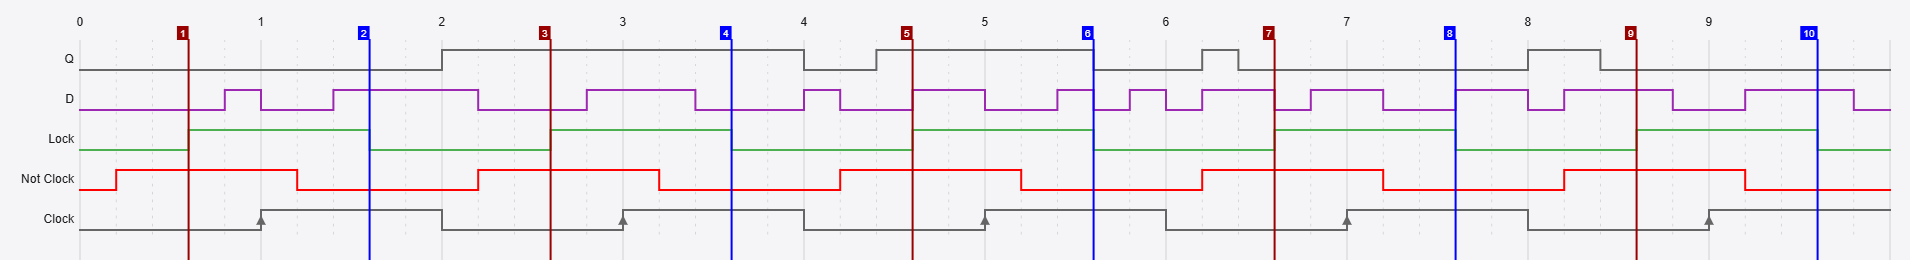
\includegraphics[width=1\linewidth]{images/D-FF-time-diagram-redstone.png}
    \caption{Diagrama temporal do flip flpo tipo D descrito}
    \label{fig:D-FF-time-diagram-redstone}
\end{figure}

O instante efetivo de captura do valor de $D$ ocorre imediatamente antes do travamento do circuito. Considerando o atraso total até o bloqueio ($t_{lock}$) e o atraso interno do repetidor ($t_{rep}$), o valor armazenado corresponde ao sinal de entrada no instante:

\begin{align*}
t &= t_{lock} - t_{rep}
\end{align*}

O instante de travamento pode ser expresso em função do clock como:

\begin{align*}
t_{lock} &= ( t_{descida}) + t_{delay} \\
&=( t_{subida} + T \cdot \text{duty cycle}) + t_{delay}
\end{align*}

Portanto, 

\begin{align*}
t &= ( t_{descida}) + t_{delay} - t_{rep} \\
&= ( t_{subida} + T \cdot \text{duty cycle}) + t_{delay} - t_{rep}
\end{align*}

onde $t_{delay}$ representa o atraso acumulado dos componentes do circuito. 

Substituindo, as variáveis para este exemplo, obtemos:

\begin{align*}
t &= t_{descida} + 1 \\
&= t_{subida} + 6
\end{align*}

Observa-se, portanto, que o instante de amostragem não coincide exatamente com a borda do clock, sendo deslocado pelos atrasos de propagação do circuito.
\label{sec:dff}
\subsection{Flip-Flop T}

O flip-flop T (\textit{Toggle}) é um elemento elemento de memória specializado na alternância de estado. Ele é amplamente utilizado na construção de contadores e divisores de frequência.

Entrada:
\begin{itemize}
    \item $T$ : Toggle
\end{itemize}

\begin{center}
\begin{tabular}{c | c}
T & $Q_{t+1}$ \\
\hline
0 & $Q_t$ \\
1 & $\overline{Q_t}$
\end{tabular}
\end{center}

Ou seja, quando $T = 1$, o estado é invertido a cada borda ativa do clock. Quando $T = 0$, o estado é mantido.

Esse comportamento pode ser expresso de forma compacta como:

\[
Q_{t+1} = T \oplus Q_t
\]

Uma forma comum de implementação do flip-flop T é a partir de um flip-flop JK, conectando-se as entradas $J$ e $K$ ao sinal $T$:

\[
J = K = T
\]

\begin{figure}[H]
    \centering
    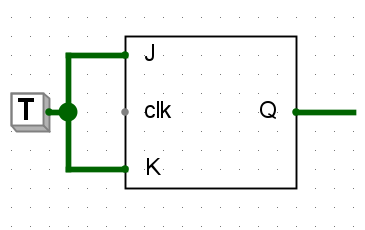
\includegraphics[width=0.5\linewidth]{images/T-FF-circuit.png}
    \caption{Implementação do Flip Flop tipo T a partir do Flip Flop JK}
    \label{fig:T-FF-circuit}
\end{figure}

Nesse arranjo, quando $T = 1$, o circuito entra no modo de alternância, enquanto $T = 0$ preserva o estado atual.

Uma aplicação fundamental do flip-flop T é como divisor de frequência. Quando $T = 1$ constantemente, o sinal de saída $Q$ alterna a cada ciclo de clock, resultando em uma frequência de saída igual à metade da frequência de entrada:

\begin{figure}[H]
    \centering
    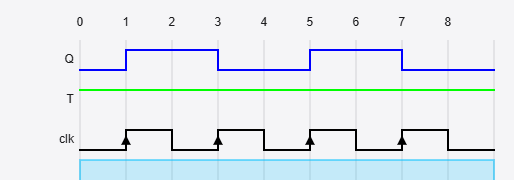
\includegraphics[width=0.8\linewidth]{images/T-FF-freq-half.png}
    \caption{Diagrama Temporal de Q por clock com $T=1$}
    \label{fig:T-FF-freq-half}
\end{figure}

\[
f_{out} = \frac{f_{clk}}{2}
\]

Além disso, esse comportamento permite a construção de contadores binários, que serão abordados na sessão \textbf{4.5}.

\begin{figure}[H]
    \centering
    \includegraphics[width=0.5\linewidth]{images/T-FF-redstone.png}
    \caption{Implementação do Flip Flop tipo T a partir do Flip Flop JK, em redstone.}
    \label{fig:T-FF-redstone}
\end{figure}
\subsection{Registradores}

Registradores são estruturas de memória compostas por múltiplos flip-flops.

\begin{figure}[H]
    \centering
    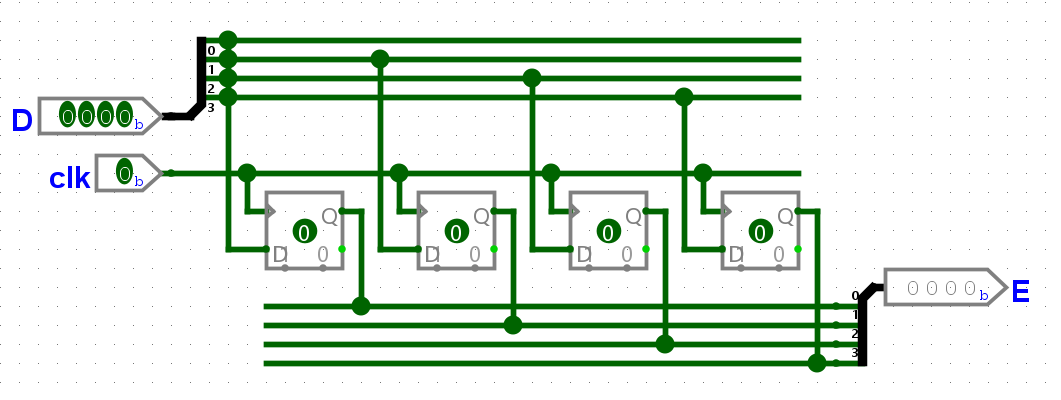
\includegraphics[width=0.8\linewidth]{images/D-Reg-4bit.png}
    \caption{Registrador de 4 bits Utilizando flip flops tipo D}
    \label{fig:D-Reg-4bit}
\end{figure}

Um registrador de $n$ bits armazena um estado $Q$ em um vetor:

\[
Q = (Q_0, Q_1, ..., Q_{n-1})
\]

De tal forma que todos os bits $Q_i \forall i \in [0, n-1]$ são atualizados simultaneamente no pulso de clock.

Esse será um componente fundamental para este projeto, visto que o estado do cronômetro, será armazenado em registradores a base de flip flops tipo D.
\subsection{Considerações sobre o Logisim Evolution}

Haja vista a importância desses elementos de memória, o Logisim Evolution possui implementações prontas em circúitos integrados, as quais serão utilizadas a partir deste ponto no documento:

\begin{figure}[H]
    \centering
    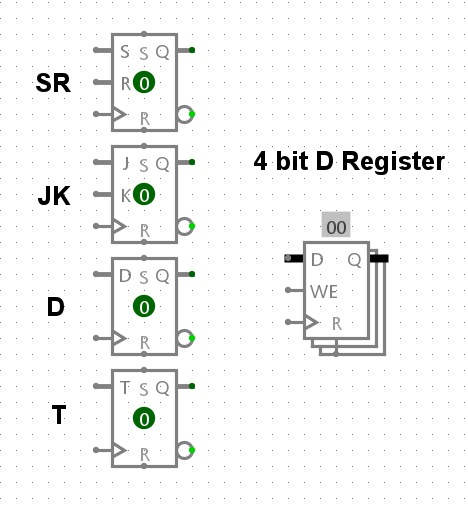
\includegraphics[width=0.5\linewidth]{images/memory-cis.png}
    \caption{Elementos de memória no Logisim Evolution}
    \label{fig:FF-logisim}
\end{figure}

Note que nesses flip flops exitem duas entradas e uma saída extras respectivamente $S, R$ e $\lnot Q$ (saída abaixo de $Q$ com circulo representando NOT).

\begin{itemize}
    \item $S_t = 1 \rightarrow Q_t = 1$, mesmo que sem pulso de clock 
    \item $R_t = 1 \rightarrow Q_t = 0$, mesmo que sem pulso de clock
    \item $S_t = R_t = 1 \rightarrow Q_t = 0$ 
\end{itemize}

Além disso, a entrada do clock é representada por: 

\begin{figure}[H]
    \centering
    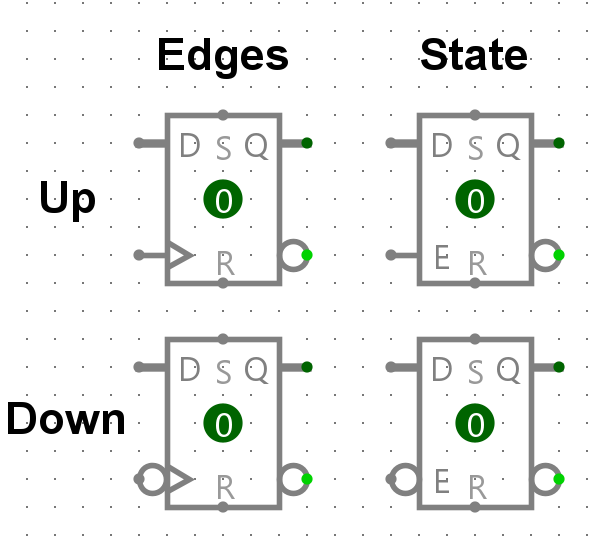
\includegraphics[width=0.4\linewidth]{images/clk-in-logisim.png}
    \caption{Representações de entrada de clock no Logisim Evolution}
    \label{fig:clk-in-logisim}
\end{figure}
